\section{Results: reproducing the paper's comparison}
\label{sec:results}

\subsection{Quantitative comparison}
Table~\ref{tab:summary} averages the four metrics over the 24 problems.
The full per-problem tables, in the paper's format (RE, ISNR, MSSIM, iterations and
the chosen parameter), are in Appendix~\ref{app:tables}.

\begin{table}[t]
\centering\small
\inputtable{tables/summary.tex}
\caption{Mean metrics over all problems. ``best ISNR/MSSIM'' counts the problems on
which a method is best among all six rows. MULTI-autoS is MULTI-auto with the
scale-aware $\epsilon$ of Sec.~\ref{sec:auto}; the Kodak rows are discussed in
Sec.~\ref{sec:kodak}. Times are medians in seconds, single-threaded,
for the final run only (parameter tuning is not included). MULTI-auto runs once with no
tuning, so its time is its entire cost, whereas the tuned methods need 10--20 runs each
to choose their parameter.}
\label{tab:summary}
\end{table}

\paragraph{MULTI vs.\ TIKH: what pixel-wise adaptivity buys.}
TIKH is exactly MULTI with a single, constant $\lambda$ (same penalty, same solver).
The difference between the two therefore isolates the effect of the
$N$ pixel-wise weights. MULTI beats TIKH on \nMainMultiBeatsTikh/\nMainN{} problems,
by \nMainMultiTikhGain\,dB ISNR on average. The gap is largest where the image
combines large flat areas with sharp structures (satellite and ct\_head under
out-of-focus blur, up to $+5$\,dB). There TIKH must choose between leaving noise
in the background and blurring the edges, whereas MULTI does not have to choose.

\paragraph{MULTI vs.\ TGV/TV: it depends on the blur.}
The comparison with the edge-preserving regularisers splits cleanly along the PSF.
\begin{itemize}[leftmargin=*,itemsep=1pt]
\item \textbf{Gaussian blur}: MULTI is the best of the four tuned methods on
  \nMainWinsGauss/\nMainNGauss{} problems, \nMainGainTGVGauss\,dB above TGV on average.
\item \textbf{Out-of-focus blur}: TGV wins on most problems, and MULTI is on
  average \nMainGainTGVOof\,dB behind it (MULTI is best on \nMainWinsOof/\nMainNOof).
\end{itemize}
This is the same pattern as in the paper's Tables~2--5, where MULTI dominates under
Gaussian blur while TGV wins several out-of-focus cases (for example
\texttt{elaine}). Per image, the mean ISNR gap MULTI$-$TGV is
\nGainTGVCthead\,dB (ct\_head), \nGainTGVCat\,dB (cat), \nGainTGVPortrait\,dB (portrait)
and \nGainTGVSatellite\,dB (satellite).
Our explanation is as follows. The out-of-focus PSF has a disk-shaped support,
so its spectrum has \emph{zeros} (rings at the zeros of the Bessel function $J_1$).
Information at those frequencies is lost and has to be \emph{filled in} by the
prior. A sparsity prior on the gradient (TV) or on the second derivative (TGV)
fills in sharp edges, which is exactly what a disk blur has destroyed. A quadratic
penalty, however locally weighted, fills them in with smooth, ringing-prone
content. The Gaussian PSF has no spectral zeros, only a smooth decay, so
nothing has to be filled in, and MULTI's smaller bias (a quadratic penalty does not shrink
contrast the way an $\ell_1$ penalty does) wins.

\paragraph{The satellite image.}
Satellite is the hardest case for MULTI. 90\% of its pixels are exactly zero (black
background), and the best $\epsilon$ is huge ($\sim\!10^{-1}$, see Sec.~\ref{sec:ablation}).
With such an $\epsilon$, MULTI behaves like TIKH in most of the image (a constant
$\lambda$), with reduced $\lambda$ only on the bright structures. TV/TGV are
better here because a piecewise-constant prior is nearly exact for this image.
The non-negativity constraint is active on a large fraction of the pixels, which
also makes the Newton Projection solver slow on this image (many backtracking steps).

\subsection{Visual study: edges and smooth regions}
Figures~\ref{fig:rest-oof}--\ref{fig:zooms} show the restorations. Two artefacts
are clearly visible. TIKH leaves grainy noise in flat regions and halos around edges.
TV makes smooth shading on the face and in the background look like flat
``cartoon'' patches. TGV and MULTI both avoid TV's staircasing. At normal viewing scale, the differences among
TV, TGV and MULTI are subtle (all are within about 1\,dB). The most visible ones are TV's
blotchy patches on the cat's fur and the portrait's forehead, and the slightly finer fur and hair
texture that MULTI keeps. The edge/flat decomposition below makes these
differences measurable.

\begin{figure}[p]
\centering
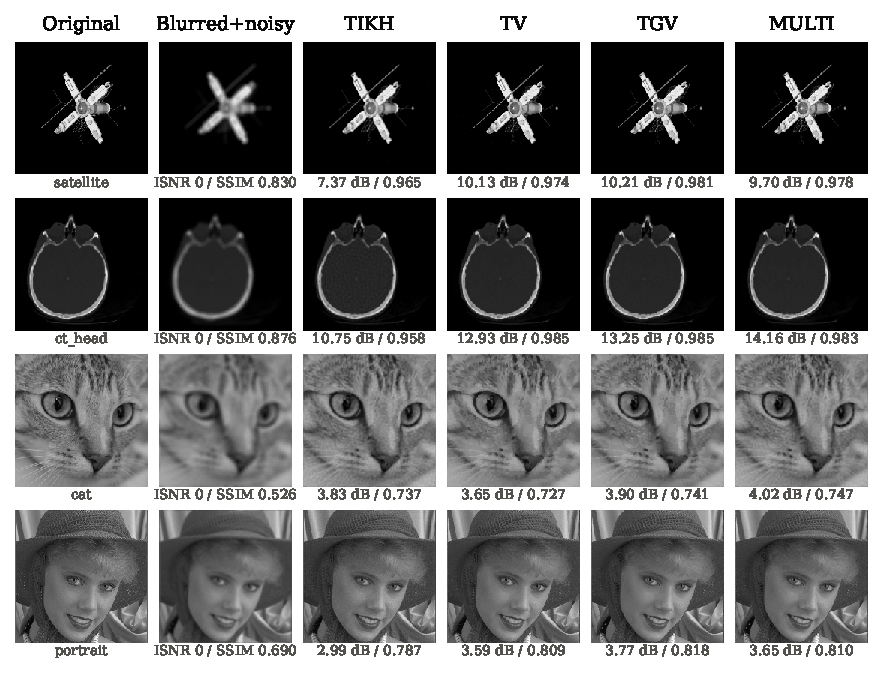
\includegraphics[width=\linewidth]{figures/restorations_oof.pdf}
\caption{Out-of-focus blur, $\delta=10^{-2}$. Below each image: ISNR (dB) / MSSIM.}
\label{fig:rest-oof}
\vspace{6pt}
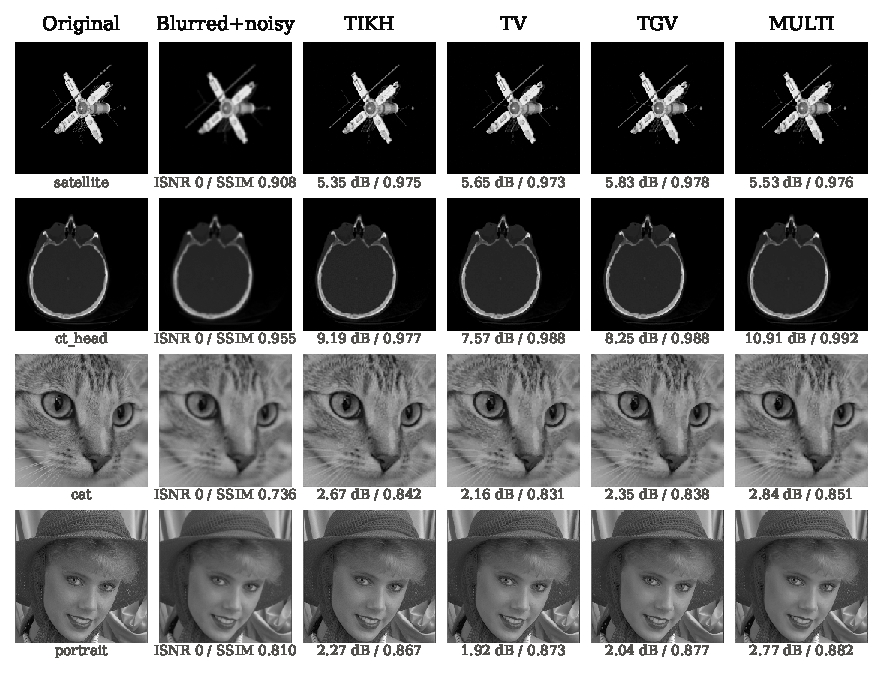
\includegraphics[width=\linewidth]{figures/restorations_gauss.pdf}
\caption{Gaussian blur, $\delta=10^{-2}$.}
\label{fig:rest-gauss}
\end{figure}

\begin{figure}[t]
\centering
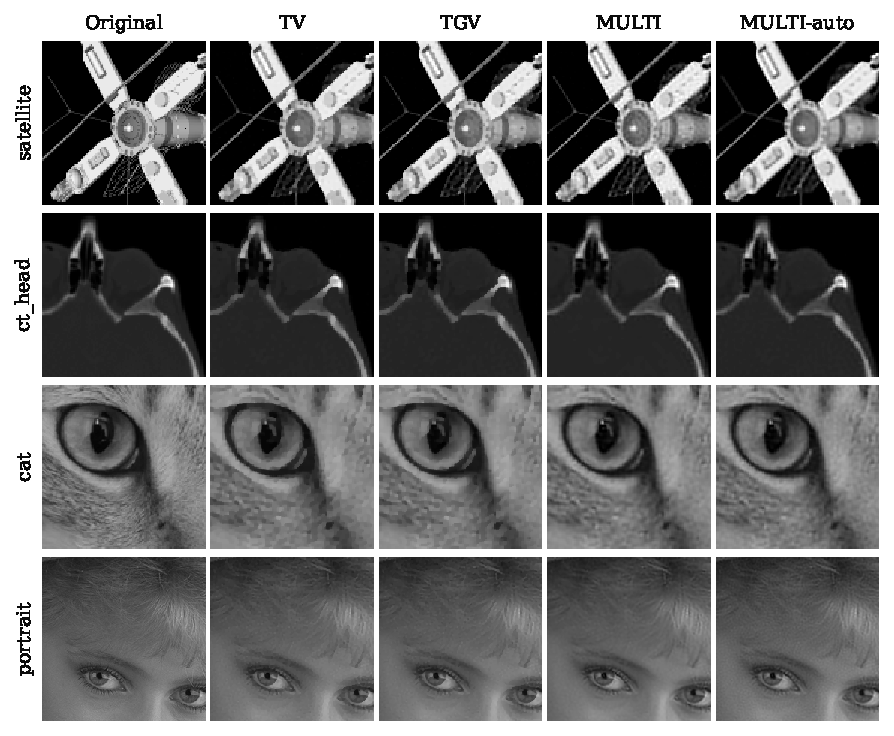
\includegraphics[width=0.9\linewidth]{figures/zooms_gauss.pdf}
\caption{Zoomed crops (Gaussian blur, $\delta=10^{-2}$). Note TV's patchy fur and forehead
texture, and the finer texture retained by MULTI.}
\label{fig:zooms}
\end{figure}

\paragraph{Edge vs.\ flat error decomposition.}
To quantify ``edges and smooth regions'', we split the pixels of every ground truth
using the smoothed gradient magnitude: the top 15\% are \emph{edge} pixels and the
bottom 50\% are \emph{flat} pixels. We then compute the RMSE of each method on each
class separately, relative to TGV (geometric mean over the 24 problems,
Fig.~\ref{fig:regions}). The result is instructive:
\begin{itemize}[leftmargin=*,itemsep=1pt]
\item TIKH and TV lose mostly in \emph{flat} regions, by
  $\times$\nFlatTIKH{} and $\times$\nFlatTV{}: noise in TIKH, and staircase patches in TV.
\item MULTI matches TGV in flat regions ($\times$\nFlatMULTI) and is
  \emph{better at edges} ($\times$\nEdgeMULTI). Its advantage comes from detail
  preservation, because low $\lambda_i$ is placed exactly where the curvature is large.
\item MULTI-auto keeps part of MULTI's edge advantage ($\times$\nEdgeAuto) but loses in
  flat regions ($\times$\nFlatAuto). At high noise its automatic $\epsilon$ is too large, so
  $\boldsymbol\lambda$ is too small and noise survives in flat areas (Sec.~\ref{sec:auto}).
\end{itemize}

\begin{figure}[t]
\centering
\begin{minipage}[t]{0.47\linewidth}\vspace{0pt}
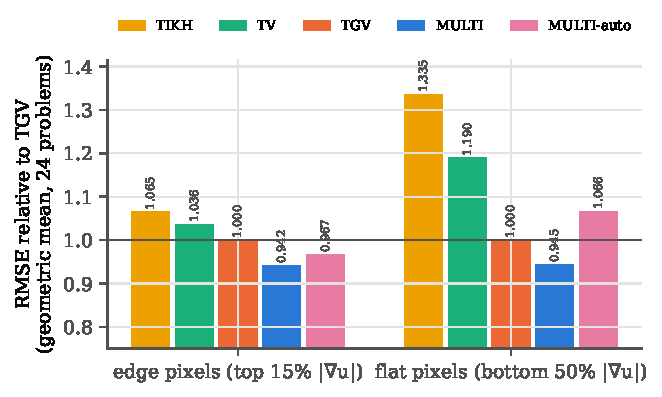
\includegraphics[width=\linewidth]{figures/region_rmse.pdf}
\caption{RMSE on edge and flat pixels relative to TGV (below 1 is better).}
\label{fig:regions}
\end{minipage}\hfill
\begin{minipage}[t]{0.5\linewidth}\vspace{0pt}
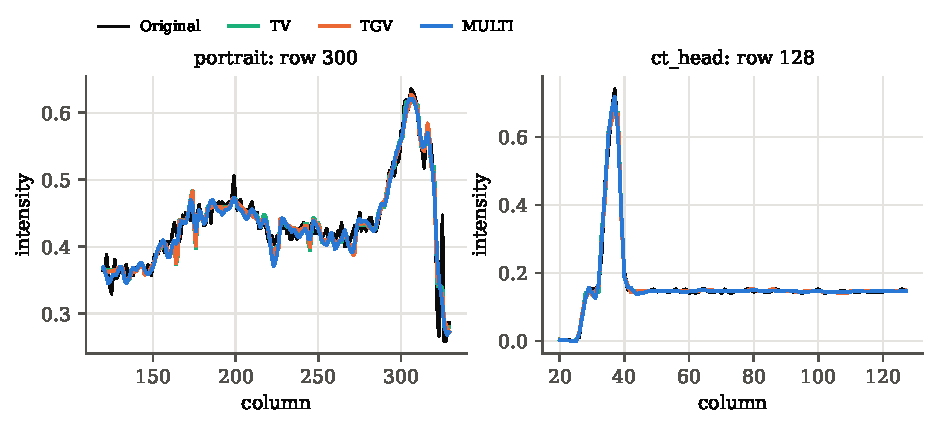
\includegraphics[width=\linewidth]{figures/profiles_oof.pdf}\\
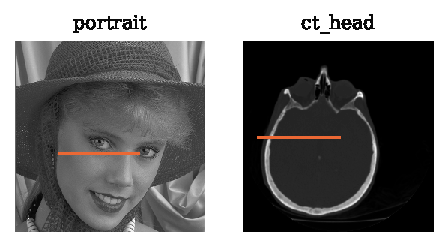
\includegraphics[width=0.75\linewidth]{figures/profiles_location.pdf}
\caption{Line profiles (out-of-focus, $\delta=10^{-2}$) and their locations.}
\label{fig:profiles}
\end{minipage}
\end{figure}

\paragraph{What the $\lambda$ map looks like.}
Figure~\ref{fig:lambda} shows the final $\boldsymbol\lambda$ of MULTI on a log scale.
It acts as an \emph{edge detector}: $\lambda_i$ is several orders of magnitude
smaller on the outlines (skull, fur pattern, hat, satellite arms) than in flat areas.
The ``thick'' outlines come from the $R\times R$ max filter, which merges the two lobes of
the Laplacian's zero crossing. In effect, MULTI performs edge detection (the course's
Laplacian/zero-crossing material) and edge-aware denoising together, inside one
variational problem.

\begin{figure}[t]
\centering
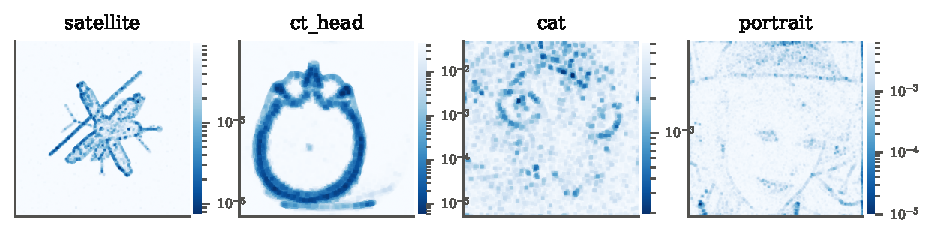
\includegraphics[width=\linewidth]{figures/lambda_maps_oof.pdf}
\caption{Final regularisation-parameter maps $\lambda_i$ of MULTI (log colour scale,
out-of-focus, $\delta=10^{-2}$). Dark means small $\lambda$, i.e.\ little smoothing.}
\label{fig:lambda}
\end{figure}

\begin{figure}[t]
\centering
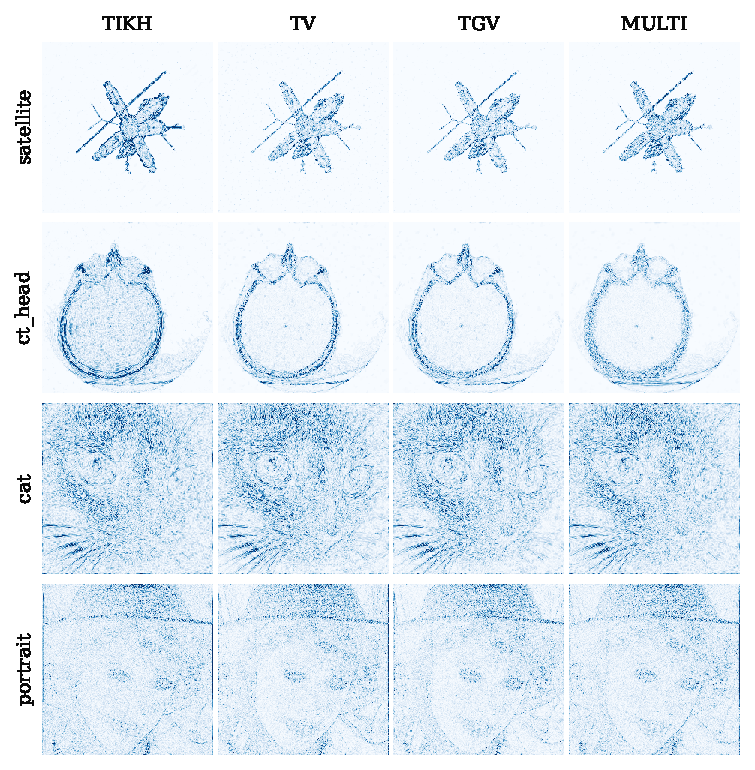
\includegraphics[width=0.8\linewidth]{figures/errormaps_oof.pdf}
\caption{Absolute error maps (out-of-focus, $\delta=10^{-2}$, common colour scale per
row). TIKH's error is spread over the flat regions; the errors of all the other methods concentrate on edges.}
\label{fig:errmaps}
\end{figure}
